%!TEX encoding = IsoLatin

%
% Chapitre "Concept retenu"
%

\chapter{Concept retenu}
\label{s:concept_retenu}

\section{Matrice de décision}

La matrice de décision du projet Fish \& Chips est présentée à la table \ref{t:matrice_decision}. Elle permet d'illustrer clairement le taux de satisfaction de tous les critères pour chaque concept afin de faire un choix éclairé. Les barèmes sont basés sur les critères du tableau \ref{t:criteres} et les pondérations sont ajustées de manière à bien refléter l'importance de chaque besoin du projet. 

\begin{table}[htp]
   \footnotesize
   \centering
   \scalebox{1.0}{
   \begin{tabular}{|c|c||c|c|c|c|}
        \hline
        Critère d'évaluation & Pond. & Concept 1 & Concept 2 & Concept 3 & Concept 4\\
        \hline
        \hline
        \textbf{Qualité du produit} & \textbf{65\%} &\textbf{ \%} &\textbf{ \%} &\textbf{ \%} &\textbf{ \%}\\
        \hline
        Résolution du capteur & 10\% & 4,9 & 8 & 3,3 & 2,4 \\
        Identification des poissons & 10\% & 9,9 & 9,9 & 9,9 & 9,9 \\
        Volume d'analyse & 5\% & 1,2 & 1,2 & 4,9 & 3,5 \\
        Capacité de stockage des données 
        & 5\% & 5 & 0,4 & 4 & 5 \\
        Durée de vie de l'alimentation du système & 5\% & 1,3 & 5 & 3,5 & 3 \\
        Acheminement des informations & 5\% & 4 & 0,5 & 3,2 & 2\\
        Fiabilité du système de sécurité & 5\% & 4,4 & 4,4 & 4,4 &  4,3 \\
        Résistance à la profondeur & 4\% & 0,6 & 0,6 & 0,5 & 2\\
        Taille des spécimens observés & 4\% & 3,7 & 3,6 & 4 & 3,4\\
        Nombre de fonctionnalités de l'alarme & 4\% & 0,9 & 0,4 & 4 & 0,4\\
        Puissance de calcul & 4\% & 2,4 & 1,3 & 1,3 & 1,3 \\
        Utilisation de l'interface graphique & 4\% & 4 & 3,2 & 1,6 & 2,4\\
        \hline\hline
        \textbf{Performance} & \textbf{20\%} & \textbf{ \%}  &\textbf{ \%} &\textbf{ \%} &\textbf{ \%} \\
        \hline
        Précision du logiciel de reconnaissance & 15\% & 13,6 & 14,3 & 5,5 & 3,6 \\
        Précision de la régulation & 2\% & 2 & 1,9 & 0,4 & 2 \\
        Précision de la mesure de température & 2\% & 2 & 1,9 & 0,4 & 1,98 \\
        Précision de la mesure du temps & 1\% & 1 & 1 & 1 & 1 \\
        \hline\hline
        \textbf{Coûts} & \textbf{15\%} &\textbf{ \%} & \textbf{ \%}& \textbf{ \%}&\textbf{ \%} \\
        \hline
        Coût de main d'oeuvre & 12\% & 0 & 0 & 1,4 & 0,9 \\
        Coûts du matériel & 3\% & 2,5 & 2,1 & 2,4 & 2,57\\
        \hline\hline
        \textbf{Total} & \textbf{100\%} &\textbf{63,4\%} &\textbf{59,7\%} &\textbf{ 55,7\%} &\textbf{51,65\%} \\
        \hline
   \end{tabular}}
    \caption{Matrice de décision du projet Fish \& Chips}
    \label{t:matrice_decision}
\end{table}




\section{Analyse de la matrice de décision}

Avec un taux de satisfaction de 63.4\%, c'est le concept 1 qui est le mieux adapté aux besoins du projet. Il se démarque surtout par sa puissance de calcul, son bon acheminement des informations et la qualité de l'interface graphique. Les concepts performance, simplicité, polyvalence et minimaliste ont respectivement des taux de satisfaction de 63.4\%, 59.7\%, 55.7\% et 51.65\%. La lacune principale du concept de performance est surtout au niveau de la durée de vie de l'alimentation. Il a été calculé selon le barème que l'alimentation parfaite est une autonomie d'une durée double que ce qui est attendu par le MFA (4 semaines) pour que le capteur fonctionne même si un oublie de maintenance survient. Or, nous avons calculé une durée de vie d'environ 2 semaines au lieu de 4 pour les batteries rechargeables, ce qui explique la piètre performance du concept 1 face au barème. Le concept 1 est donc retenu et fait l'objet d'une analyse plus détaillée à la section \ref{ch7:concept_retenu}.

\section{Description du concept retenu}
\label{ch7:concept_retenu}

\textbf{Prise de mesure}
\begin{itemize}
    \item Prise d'image à l'aide du senseur OV5640
    \item Mesure de la température par diode 1n4148
    \item Mesure de la date et heure par l'utilisation des méta-données
\end{itemize}

\textbf{Support physique}
\begin{itemize}
    \item Compilation des données avec l'ordinateur personnalisé
    \item Alimentation à l'aide de batteries rechargeables
    \item Régulation de la température par Module Peltier
    \item Stockage de données par cloud hubiC
    \item Acheminement des informations manuelle
\end{itemize}

\textbf{Logique de programmation}
\begin{itemize}
    \item Identification par réseau de neurone convolutionnel
    \item Sécurité par clés d'encryption
\end{itemize}

\textbf{Communication}
\begin{itemize}
    \item Interface graphique avec CodeCreators
    \item Notifications Amazon SNS
\end{itemize}

\clearpage

\subsection{Prise de mesure}
Dans l'optique de la prise des mesures sous l'eau, on utilisera le capteur OV 5640. Ce capteur d'image n'est pas celui avec la meilleure résolution, mais remplit la totalité des exigences du client. C'est la petite taille de pixel agencé avec la focale qui permet d'imager des poissons avec une bonne résolution. Son avantage par rapport aux autres caméras vient du fait qu'elle est entièrement programmable à l'aide d'un ordinateur Raspberry Pi auquel on y a ajouté une diode électroluminescente pour l'éclairage nocturne. De plus, elle est beaucoup moins coûteuse, de petite taille et disponible à un faible coût. De ce fait, ce capteur semble le plus adapté pour les besoins du Ministère.
\vspace{5mm}

Pour mesurer la température à l'intérieur et à l'extérieur du capteur, on utilise un Raspberry Pi connecté à une thermistance. Cet assemblage permet de mesurer à peu de frais avec une grande précision les températures que le client souhaite connaître.
\vspace{5mm}

De plus, afin de déterminer les moments où les images sont prises, on utilise une identification par les méta-données des fichiers. Grâce à ce concept de programmation, on pourra facilement savoir à quels moments quelles images ont été prises. Cet outil est très intéressant dû au fait qu'il soit précis à la seconde près et que son implémentation soit très simple.
\vspace{5mm}


\subsection{Support physique}
Ensuite, pour supporter et analyser les données disponibles, on utilisera le matériel informatique disponible dans l'ordinateur personnalisé. Grâce à cet ordinateur, un code plus complexe pourra être exécuté et l'entraînement du logiciel de reconnaissance sera efficace. Ensuite, grâce au code, toutes les informations seront traitées et organisées de façon à créer les vignettes et stocker les informations importantes aux yeux du client (date, heure, température, type de poisson, etc.).
\vspace{5mm}

De plus, par l'alimentation avec les batteries rechargeables Energizer Recharge Power Plus, il sera possible de fournir à notre machine une puissance électrique suffisante pour alimenter le capteur et assurer son fonctionnement sur une durée de 2 semaines. Comme elles sont rechargeables, il est possible de ne pas avoir à en racheter d'autres sur la durée de l'utilisation du capteur. Avec deux ensembles de batteries, il sera également possible d'effectuer un roulement et préserver la qualité des batteries plus longtemps.
\vspace{5mm}

Le boîtier étanche permet de protéger l'ensemble des composantes électroniques de l'eau. Son design est fait pour minimiser la masse tout en optimisant sa résistance et son volume. Sa fenêtre encastrée en PMMA permet de voir au travers du boîtier tout en résistant à la pression.
\vspace{5mm}

Comme le système consomme de la puissance électrique, la machine aura besoin d'un système de refroidissement pour évacuer la chaleur et empêcher au système d'être en état de surchauffe, ce qui pourrait endommager la machine et causer des problèmes lors de la prise des mesures. L'avantage d'un module programmable comme le Raspberry Pi est qu'il est ensuite plus facile d'implémenter une régulation de la température. La grande précision de la mesure de la température combinée à l'efficacité du module Peltier offre une régulation optimale. Cette partie du système se procure très facilement pour un prix d'une vingtaine de dollars.
\vspace{5mm}

Afin de stocker toutes les données qui seront accumulées tout au long de la durée d'utilisation de la machine, nous utiliserons l'informatique de nuage fournie par la compagnie hubiC d'une capacité de stockage de 10 To. Une carte SD sera également nécessaire pour effectuer le transfert de la prise de données de la caméra au nuage avec l'ordinateur personnalisé comme intermédiaire. Pour contenir ces données sur une durée estimée de deux ans, nous pourrons sauvegarder toutes les données tel que souhaité par le client.
\vspace{5mm}

Enfin, pour acheminer les informations, cela sera fait de façon manuelle comme introduit précédemment: lorsque le capteur sera retiré au bout de 14 jours, il sera possible de retirer les données capturées par la caméra sur la carte SD, les entreposer temporairement sur l'ordinateur personnalisé et mettre à jour la plateforme hubiC.
\vspace{5mm}

\subsection{Logique de programmation}

Lors de la capture des images, il a été exigées par le client de déterminer de quels poissons il s'agissait sur l'image. Pour accomplir cette mission, il a été décidé d'utiliser un réseau de neurones convolutionnel avec la librairie Tensorflow. Ces outils informatique entraînés à l'identification des poissons du Québec pourront, dès l'image capturée, déterminer l'espèce du poisson et le tout pourra être stocker avec le disque SSD.
\vspace{5mm}

\subsection{Communication}

L'interface graphique choisie est la plateforme fournie par CodeCreators. Cela inclut la base de données où toutes les vignettes seront enregistrées. De plus, cela inclut l'interface où il sera possible d'ajuster les différents paramètres de la caméra via le Raspberry Pi. En effet, dans un contexte où il faut être capable de prendre des photos nocturnes, il peut être intéressant d'ajuster l'ISO, le focus et la durée d'exposition. C'est sur cette interface que l'utilisateur pourra regarder les différentes statistiques des poissons, et ce, en tout temps puisqu'il s'agit d'une application web. CodeCreators offre une plateforme qui est reconnue pour produire des interfaces faciles d'utilisation et même accessibles à partir d'un téléphone mobile. Il sera toujours possible d'accéder à distance au capteur avec une connexion SSH sécurisée d'un quelconque ordinateur possédant les droits d'accès au Raspberry Pi.
\vspace{5mm}

La plateforme Amazon SNS permet d'envoyer des notifications et avertir un opérateur en cas de problème dans l'identification des poissons, l'alimentation du capteur ou la régalution de la température. Avec Amazon SNS, il est possible d'envoyer des notifications par email, sur un téléphone intelligent et un appareil de bureau et par SMS pour en avertir l'opérateur le plus rapidement possible. De plus, il serait possible de coupler cette composante avec l'application web.


\section{Conclusion}

L'équipe des Requins était chargé de fournir le design conceptuel du projet Fish \& Chips, un système autonome fixe chargé du comptage et de l'identification de la faune marine. Une démarche prescriptive à été effectuée afin de répondre à l'ensemble des besoins du Ministère de la Faune Aquatique. Le problème a été analysé de manière exhaustive pour proposer, au final, un concept de solution qui réponds aux critères du client.
\vspace{5mm}

Les besoins du MFA ont d'abord été examinés afin de discerner correctement les problèmes du projet. Les objectifs ainsi découlés ont permis de définir différents critères qui reflètent les attentes du client. Chacune des fonctions du système propose quatre solutions distinctes afin de fournir au client une panoplie d'options. Ces solutions, regroupées en quatre concepts, ont été évaluées selon des barèmes appropriés pour proposer au MFA un concept unique qui respecte ses besoins. Les concepts ont ainsi été comparés selon leur taux de satisfaction par rapport aux critères. De ces quatre concepts, un seul a été retenu et se distingue de ses pairs par sa performance.

 
 
 
    
\begin{figure}
        \centering
        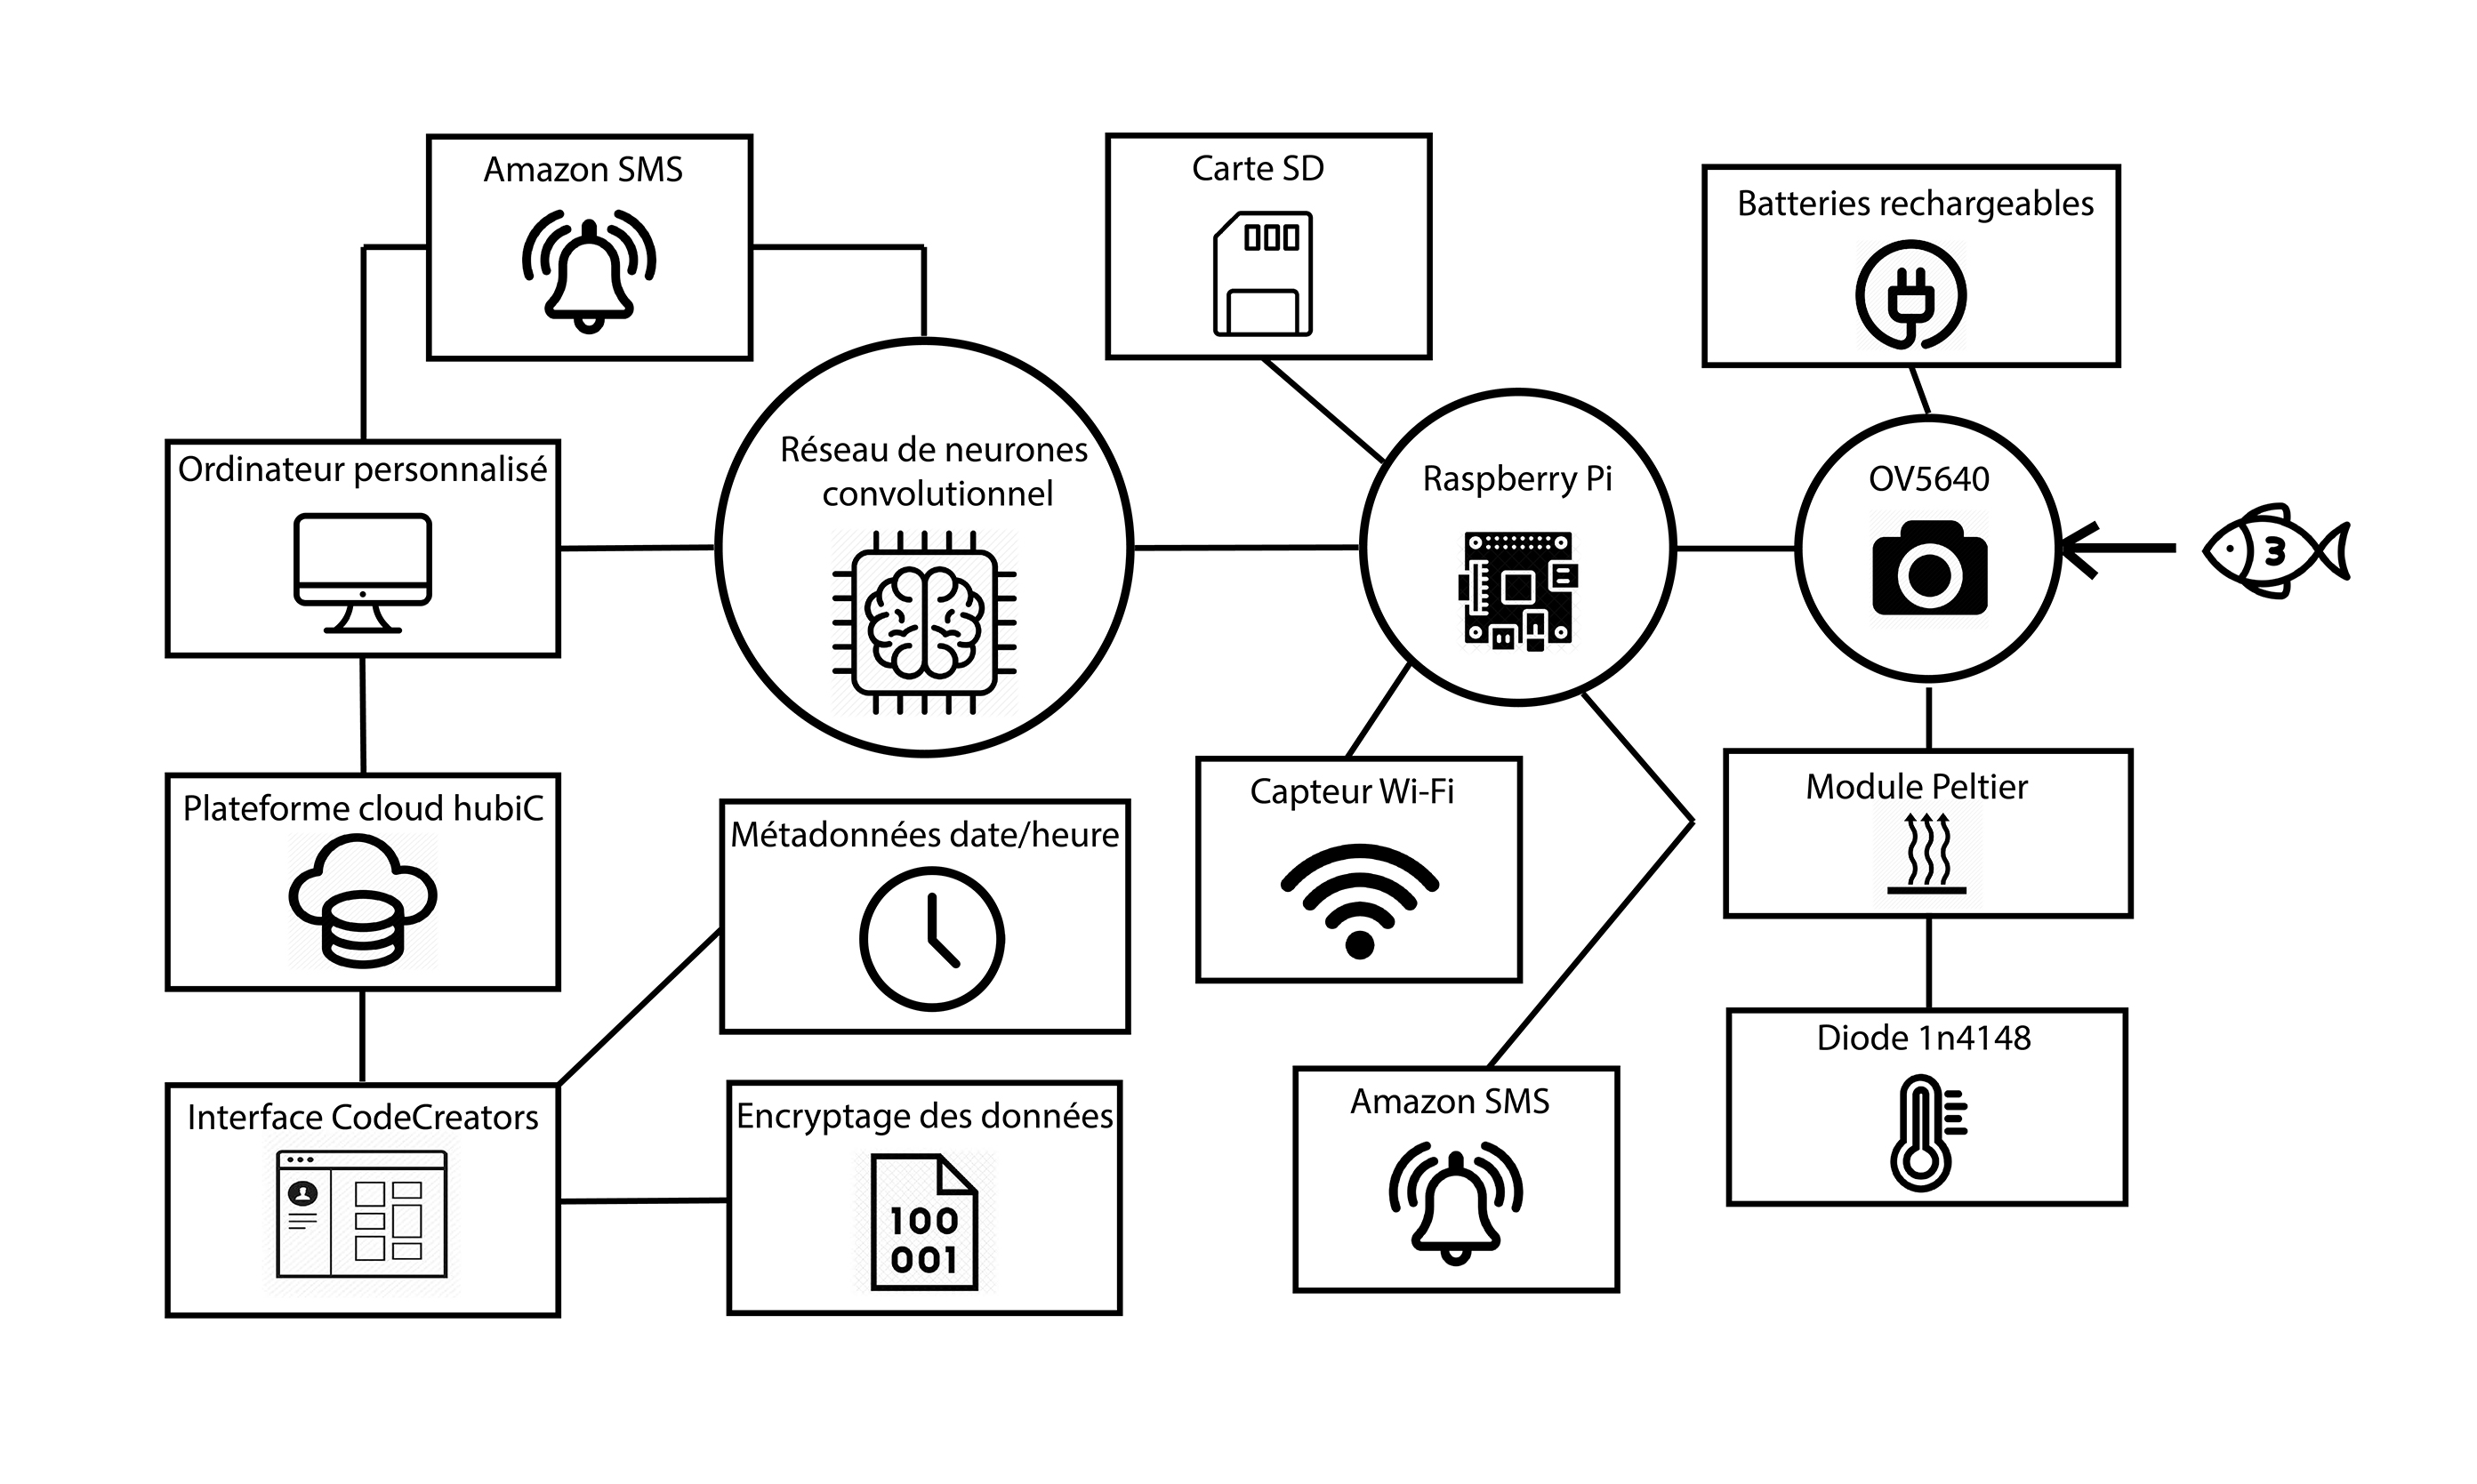
\includegraphics[width=\linewidth]{fig/schema_designnnnnn.jpg}
        \caption{Diagramme physique de la solution retenue pour le projet Fish \& Chips}
        \label{fig:concept_retenu}
\end{figure}

